%
%
%
\clearpage
\section{Simulation setup}
\label{sec:setup}

Two different simulation setups are used, in order to systematically provide an
independent cross-check of the expected results for the performance of
HGCal:

\begin{itemize}
\item stand-alone simulation of a simplified geometry using a calorimeter stack detector with a transverse size of $20 \times 20\cm^2$
\item cylindrical endcap geometry integrated within an extended upgrade scenario within CMSSW.
\end{itemize}

In both cases alternative analysis are run in parallel and cross-check
each other systematically.
In the following sections we describe in more detail each simulation setup.

%%
%%
%%
\subsection{Stand-alone simulation setup}
\label{subsec:standalone}

The stand-alone setup is used for three different purposes:

\begin{enumerate}
\item provide a quick handle to optimise the design parameters (see later Sec.~\ref{sec:optim})
\item extract performance results in ideal conditions
\item cross-check the performances in pileup conditions with the CMSSW setup
\end{enumerate}

The implementation, based on \GEANT 4 v9.6.2, is fully available in git~\cite{G4git}.
In our simulation we use the so-called QGSP\_FTFP\_BERT physics list.
To avoid infrared divergence, some electromagnetic processes require a
threshold below which no secondary will be generated.
If at a given step the particle is not expected to travel longer than
the threshold cut it is forced to yield all its energy to the medium.
In the case of electromagnetic showers the appropriate choice of these
cuts is crucial in order not to generate excess of $\delta$-like
deposits in the sensitive volumes.
We set the range cuts to be 10\mum for electrons, positrons and photons in all silicon volumes
and 1\mm elsewhere.
For reference, when considering 700\mum in Si, a 420\keV (5.8\keV) electron (photon) would deposit all its energy in
one step. With the reduced 10\mum, the energy threshold lowers to 32\keV
for electrons and 990~eV for photons.

Most materials are assumed to be default in \GEANT 4 except the
Printed Circuit Board (PCB) material which is defined as the G10
admixture
composed of Si, O, C and H in the proportions 1:2:3:3 with a density of 1.7g/\cm$^3$.

The baseline setup is described in Table~\ref{tab:baselinesampling}
and it consists of 3 sampling sections, each composed of 10 layers
with increasing absorber radiation lengths in the proportion 1:1.6:2.4.
This setup is expected to provide fine grain sampling of the early
stages of shower development where statistical fluctuations
dominate. Coarser sampling is used near the shower maximum (for
$E>5\GeV$) without compromising the expected resolution.
In the later stage of the shower development, expected to be dominated
by halo contributions, the sampling is furthermore increased.
This baseline setup is expected to provide optimal performance given the
constraints imposed by the operation under the expected HL-LHC
conditions as it will be described later in this manuscript.

\begin{table}[h!]
 \begin{center}
\caption{\label{tab:baselinesampling} 
Layout of the baseline sampling ECAL calorimeter. 
For each section the number of layers and material budget of each
material per layer is quoted.
The total material budget of a section is given in the rightmost
column in units of radiation lenghts.
}
\begin{tabular}{cccccccc}
\hline
\multirow{2}{*}{Section} & \multirow{2}{*}{Layers} & \multicolumn{5}{c}{Material thickness/layer (\mm)} & Total budget \\
& & Pb & Cu & Si & PCB & Air &  (1/\Xnot)\\\hline\hline
A & 0-9  & 1.63 & 3 & 0.2 & 1 & 2 & 5\\
B & 10-19 & 3.32 & 3 & 0.2 & 1 & 2 & 8\\
C & 20-29 & 5.56 & 3 & 0.2 & 1 & 2 &  12 \\
\hline
\end{tabular}
\end{center}
\end{table}

Figure~\ref{fig:g4vis} shows an event display of a 50\GeV electron
shower transversing the baseline geometry detailed in
Table~\ref{tab:baselinesampling}.

\begin{figure}[h!]
  \begin{center}
    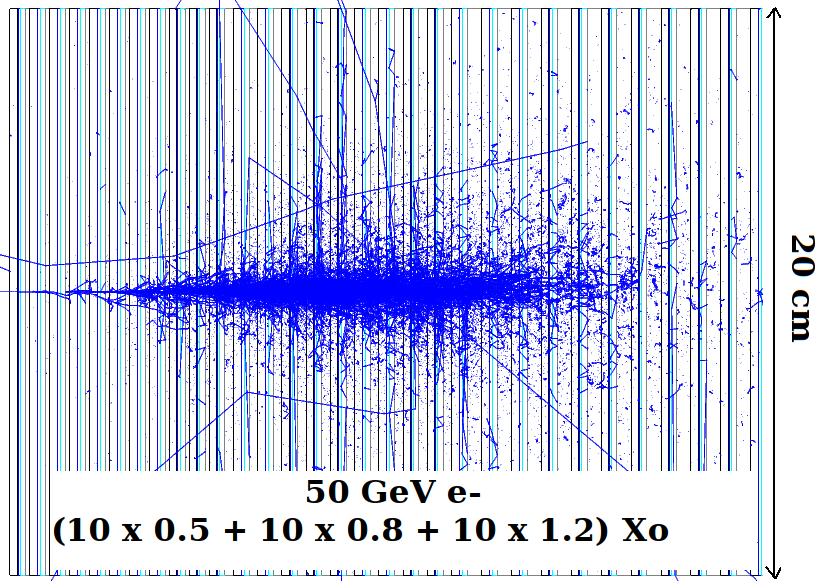
\includegraphics[width=0.6\textwidth]{figures/e_50GeV_concept_v3.png}
    \caption{Event display of a 50 GeV electron showers in the
      standalone simulation. Thirty layers in three blocks of different
      thicknesses are used as the calorimeter model (cf. Table~\ref{tab:baselinesampling}). 
      Electron deposits are shown in blue. Photons have been hidden
      for better visualisation.}
    \label{fig:g4vis}
  \end{center}
\end{figure}

Different detector layouts are studied as well, with the goal of comparing with the
baseline described above. In these setups we introduce minimalistic
changes to the setup with the goal of testing sensitivity to different
characteristics of the development of electromagnetic showers.
Table~\ref{tab:variantsamplings} summarizes the characteristics of
these alternative setups.

\begin{table}[h!]
 \begin{center}
\caption{\label{tab:variantsamplings}
Alternatives to the baseline tested in the stand-alone simulation. For
each variant the minimal changes introduced with respect to baseline
setup described in Table~\ref{tab:baselinesampling} are quoted.
}
\hspace*{-0.5cm}
\begin{tabular}{llc}
\hline Variant & Description & Code in simulation \\\hline\hline
Si *\mum & *=80,120,500\mum used for the Si thicnkess & v\_HGCALEE\_Si*\\\hline
Gap *\mm & Air gaps of *=1,4\mm are considered & v\_HGCALEE\_gap*\\\hline
Inverted & Sampling sections A and B are reversed in order & v\_HGCALEE\_inverted\\\hline
\multirow{2}{*}{W} & W absorber is used with 0.7, 2.1 and 3.5\mm  & \multirow{2}{*}{v\_HGCALEE\_W} \\
& thicknesses for sections A,B,C correspondingly & \\\hline
CALICE & simplified version of the CALICE detector using 500\mum~\cite{CALICE} & v\_CALICE\\\hline
CALICE-like & baseline variant with 1.304\mm Pb thickness for section A & v\_HGCALEE\_CALICE\\\hline
\multirow{2}{*}{Concept} & baseline with extra Cu+Si+Pad+Air section & \multirow{2}{*}{v\_HGCALEE\_concept} \\
& added in front of section A & \\
\hline
\end{tabular}
\end{center}
\end{table}


%%
%%
%%
\subsection{CMSSW setup}
\label{subsec:cmssw}


\FIXME{Expand on the relevant CMSSW releases, packages affected, and
  geometry scenarios.}

\FIXME{Describe current DetId and numbering schemes.}

\FIXME{Add event display.}

